\documentclass[conference]{IEEEtran}
% \usepackage{cite}
% \usepackage{amsmath,amssymb,amsfonts}
% \usepackage{algorithmic}
\usepackage{graphicx}
\usepackage{multirow}
\usepackage{booktabs}
\usepackage[font=small]{caption}
\usepackage{subcaption}
% \usepackage{textcomp}
% \usepackage{xcolor}
\graphicspath{{./images/}}
\def\BibTeX{{\rm B\kern-.05em{\sc i\kern-.025em b}\kern-.08em
    T\kern-.1667em\lower.7ex\hbox{E}\kern-.125emX}}
\begin{document}
\captionsetup[table]{
    justification=centerlast,
    labelsep=newline,
    textfont={footnotesize, sc},
    labelfont=footnotesize,
    skip=0pt,
}

\title{Shallow Convolutional Neural Network Architectures for Music Genre Classification}

\author{\IEEEauthorblockN{George Herbert}
\IEEEauthorblockA{\textit{Department of Computer Science} \\
\textit{University of Bristol}\\
Bristol, United Kingdom \\
cj19328@bristol.ac.uk}
}

\maketitle

\begin{abstract}
This paper describes a reimplementation of the shallow convolutional neural network architecture proposed by Schindler et al. in \cite{SchindlerLidyRauber} for music genre classification.
The first part of the paper focuses on the reimplementation details and provides an extensive analysis of the network's performance.
The latter part of the paper builds on the work of Schindler et al., showing that the inclusion of two batch normalisation layers substantially improves performance.
\end{abstract}

\begin{IEEEkeywords}
Music Information Retrieval, Music Genre Classification, Convolutional Neural Networks
\end{IEEEkeywords}

\section{Introduction}

The explosive growth of digital music platforms has sparked significant advancements in the field of music information retrieval (MIR).
This rapidly evolving discipline focuses on developing computational techniques to extract valuable insights from music and audio signals.
As MIR technologies continue to advance, they are becoming increasingly crucial for the music industry, enabling the creation of more effective tools, such as recommender systems, which can provide a competitive edge in a crowded market.

One of the critical challenges in MIR is genre classification, which involves identifying the musical genre of a given audio signal.
Accurate genre classification can help music providers organise and categorise their catalogues, enabling users to search and discover new music more efficiently and effectively.
Early efforts to solve this problem, such as that proposed by Tzanetakis and Cook \cite{TzanetakisCook}, employed statistical classifiers trained on vector summaries of features such as timbral texture, rhythmic content and pitch content.
However, these summaries fail to capture the temporal structure of the underlying audio.
In recent years, researchers have turned to audio spectrograms, which represent frequency data over time, to train state-of-the-art deep-learning models that can effectively classify audio signals based on genre.

Convolutional neural networks (CNNs) are one type of network that has been widely employed, following their successes in computer vision.
In this paper, we explore the use of CNNs for genre classification and specifically investigate the shallow CNN architecture proposed by Schindler et al. in \cite{SchindlerLidyRauber}, which they showed to achieve modest performance in this task.

\section{Related Work}

This section summarises some of the recent state-of-the-art approaches to genre classification.

Liu et al. \cite{LiuFengLiuWangLiu} recently proposed a novel architecture named a Bottom-up Broadcast Neural Network (BBNN) to deal with some problems traditionally associated with genre classification.
They identified that many previously developed architectures had focused on abstracting high-level semantic features layer-by-layer; as a result, these architectures suffer from a considerable loss of lower-level features, which are critical to genre classification.
Thus, Liu et al. specifically designed the BBNN architecture to deal with this problem by introducing the novel Broadcast Module (BM), which uses Inception modules connected by dense connectivity.
The Inception modules contain parallel convolutional and max pooling layers of varying shapes, thus enabling the network to capture temporal and spectral hierarchies at multiple scales.
The dense connectivity enables the low-level information extracted from the earlier modules to be propagated throughout the network.
Liu et al. demonstrated that the BBNN achieves state-of-the-art performance on various music datasets.

One of the main problems in the wider MIR domain is the lack of the large training datasets that are frequently required to train powerful deep neural networks.
To deal with this problem, Hung et al. \cite{HungYangChenLerch} very recently published a novel method known as input-dependent neural model reprogramming (ID-NMR).
ID-NMR is a transfer learning training scheme that leverages pre-trained models from a source domain and applies it to a target domain.
Hung et al. successfully applied this technique to transform two models trained on speech and audio data to genre classification.
Their model outperformed both a fine-tuning transfer learning method and existing state-of-the-art models pre-trained on music-specific datasets.

\section{Dataset}

To train and evaluate the models in this study, I used the GTZAN dataset, compiled by Tzanetakis and Cook \cite{TzanetakisCook}.
GTZAN is a balanced dataset, containing 100 tracks for each of the ten genres labelled: blues, classical, country, disco, hip-hop, jazz, metal, pop, reggae and rock.
The dataset contains 1000 WAV audio tracks, each 30 seconds long.

I utilised a stratified-by-genre split to produce a training and test set: the training set consisted of 750 tracks (75 tracks from each genre), while the test set contained the remaining 250 tracks.

\section{CNN Architecture}

\begin{figure}[htbp]
    \centerline{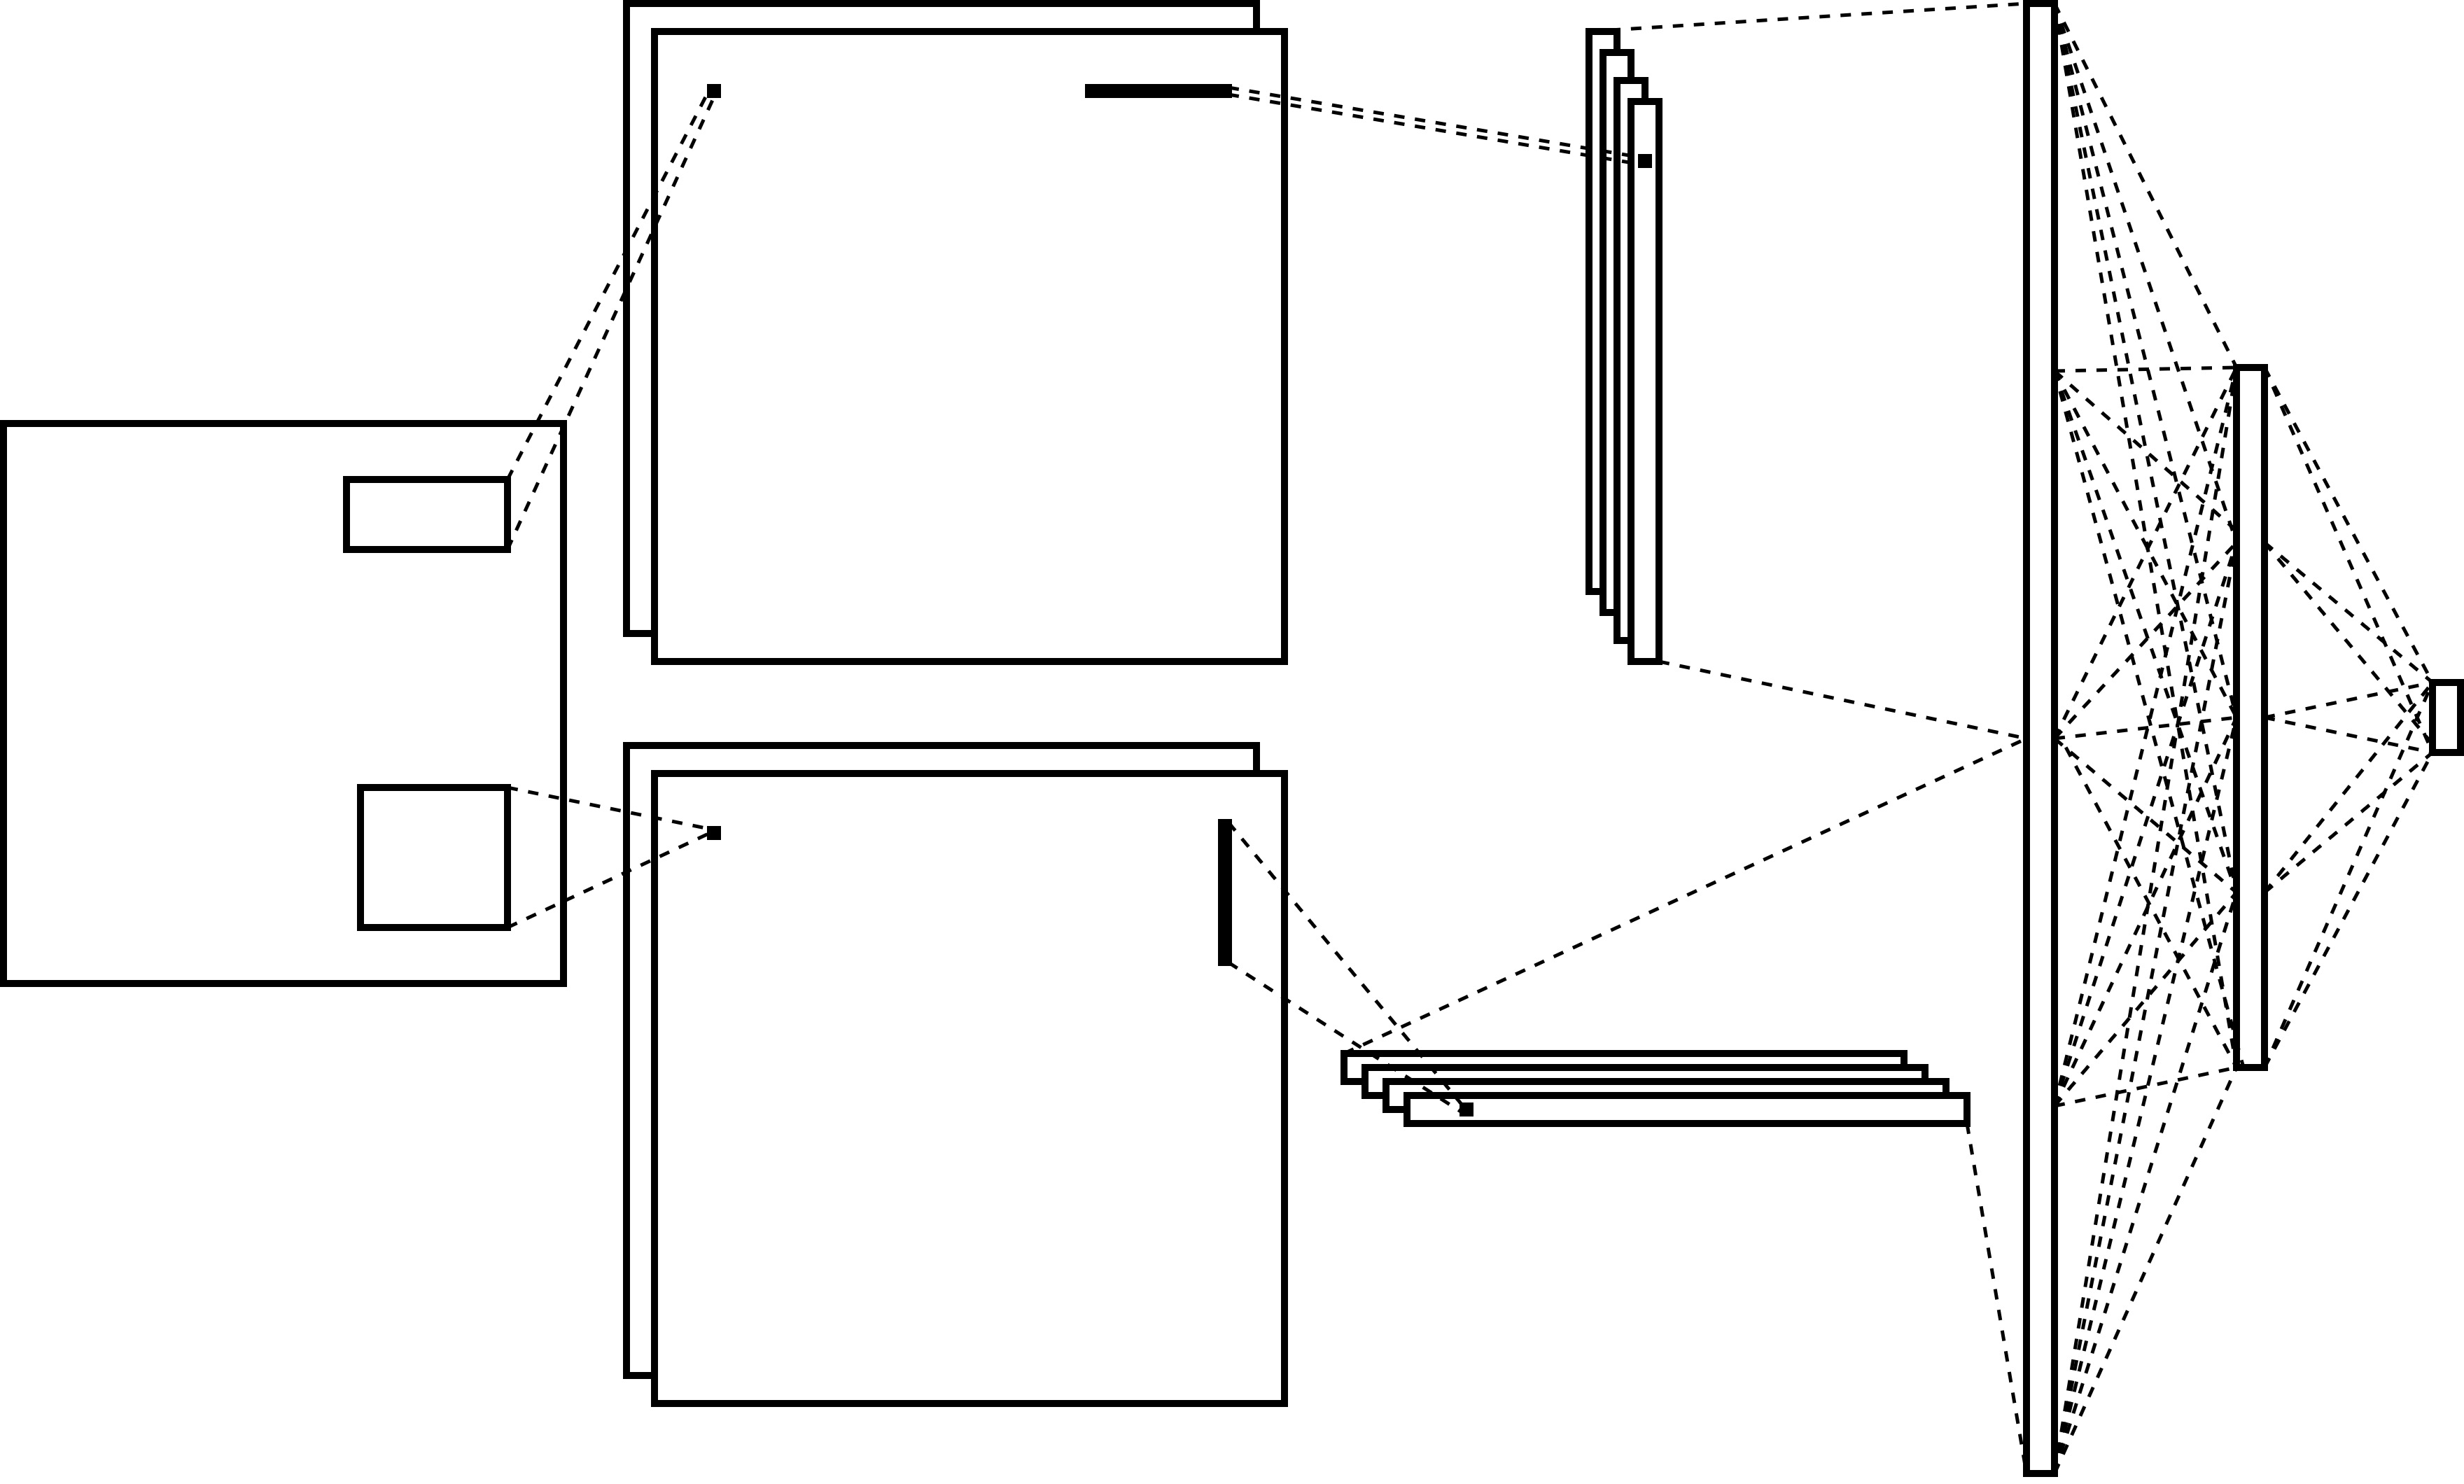
\includegraphics[width=\columnwidth]{architecture.jpg}}
    \caption{Schematic representation of the shallow CNN architecture as described by Schindler et al. in \cite{SchindlerLidyRauber}.}
    \label{architecture}
\end{figure}

I recreated the shallow CNN architecture described by Schindler et al. in \cite{SchindlerLidyRauber}.
Figure \ref{architecture} displays a schematic representation of the architecture.
The network takes log-mel spectrograms of shape $80\times80$ as input, of which the dimensions correspond to frequency and time.
The architecture employs a parallel design to effectively process the temporal and spectral characteristics of the input spectrograms.
The upper pipeline captures frequency relations in the input, while the lower pipeline captures temporal relations.

The upper pipeline includes a convolutional layer with 16 kernels of shape $10\times23$ (with padding), which produces 16 square feature maps of shape $80\times80$.
These feature maps are then downsampled using a max pooling layer with a window of shape $1\times20$, resulting in 16 vertical rectangular feature maps of shape $80\times4$.
The lower pipeline includes a convolutional layer with 16 kernels of shape $21\times20$ (with padding).
The resulting 16 square feature maps of shape $80\times80$ are downsampled using a max pooling layer with a window of shape $20\times1$, resulting in 16 horizontal rectangular feature maps of shape $4\times80$.

The 16 feature maps from each pipeline are flattened and concatenated to a shape of $1\times10240$, which is mapped to a 200-neuron fully-connected layer.
These final 200 neurons are then mapped to ten output neurons, with a 10\% dropout utilised to mitigate overfitting.
The softmax function is applied to these ten output neurons to produce a pseudo-probability distribution that indicates the probability that a given input belongs to each of the ten genres.

Except for the final layer, each convolutional and fully-connected layer is passed through a Leaky ReLU activation function with $\alpha=0.3$.
Leaky ReLU is an extension to the ReLU activation function that outputs a small non-zero value $f(x) = \alpha x$ for negative inputs.

\section{Implementation Details}

\subsection{Preprocessing}

A preprocessing stage converted the original audio files in the GTZAN dataset into 15000 log-mel spectrograms for training and evaluation. 
Each audio track in the dataset was first split into chunks of approximately 0.93 seconds, using a step size of 50\%.
Fifteen randomly selected chunks from each track were then transformed into log-mel spectrograms of shape $80\times80$ using a fast Fourier transform with a window size of 1024, and a step size of 50\%.

The tracks were split into training and test sets before the spectrograms were generated to avoid data leakage, thus ensuring that the model did not have access to any information about the test set during training, allowing for a fair and accurate evaluation of its performance.

\subsection{Training Details}

I constructed and trained the CNN using Python and the PyTorch \cite{PyTorch} machine learning framework and implemented the training method described by Schindler et al. in \cite{SchindlerLidyRauber}.
I used the cross-entropy loss function to evaluate the network's performance and employed L1 regularisation with a penalty value of $0.0001$ to mitigate overfitting.
I used the Adam optimiser \cite{KingmaBa}---an extension of stochastic gradient descent---to optimise the network, using a learning rate of $5\times10^{-5}$, $\beta_1=0.9$, $\beta_2=0.999$, and $\epsilon=1\times10^{-8}$ for numerical stability.
I trained the network on a BlueCrystal Phase 4 GPU node containing two NVIDIA Tesla P100 GPUs \cite{bc4}.

\subsection{Weight initialisation}

Weight initialisation is a crucial design choice, as it determines the starting point of the optimisation procedure.
In the shallow CNN architecture proposed by Schindler et al. in \cite{SchindlerLidyRauber}, the authors did not specify their weight initialisation procedure.
However, there are modern heuristics for weight initialisation that depend on the activation function used in the network.
Since the network uses the Leaky ReLU activation function throughout, I implemented He Gaussian initialisation, which is well-suited.

\subsection{Batch size}

Batch size is a vital hyperparameter to consider when training deep learning models.
Smaller batches give rise to longer epochs and introduce extra noise to the weight updates; however, this noise can prove beneficial if the error manifold has many deep local optima.
Conversely, larger batches give rise to shorter epochs, but networks trained with large batches often struggle to generalise.
Schindler et al. did not identify the batch size they used for training in \cite{SchindlerLidyRauber}.
Therefore, I experimented with multiple batch sizes in preliminary experiments and found that a batch size of 64 yielded the best results.

\section{Replicating Quantitative Results}

Table \ref{shallow_results} shows the mean accuracy of the implementation on the test set over five runs, along with the accuracy achieved by Schindler et al. \cite{SchindlerLidyRauber} for comparison.
The results differed by approximately 3\%, likely due to differences in the experimental setup and assumptions made between the two studies.

\begin{table}[htbp]
    \caption{Accuracy achieved on the test set}
    \begin{center}
    \begin{tabular}{l c c}
    \toprule
    \textbf{Model}&\textbf{Epoch}&\textbf{Accuracy}\\
    \midrule
    \multirow{ 2}{*}{My CNN} & 100 & 63.28 \\
    & 200 & 64.22 \\
    \midrule
    \multirow{ 2}{*}{Schindler et al.} & 100 & 66.56\\
    & 200 & 67.49 \\
    \bottomrule
    \end{tabular}
    \label{shallow_results}
    \end{center}
\end{table}

Figure \ref{confusion_matrix} is a confusion matrix displaying the performance of the implementation after 200 epochs.
Notably, the matrix shows a significant difference in the per-class accuracy for different genres.
For example, the network achieved a high per-class accuracy of at least 80\% in the blues, classical and metal genres.
While conversely, it achieved less than a 50\% per-class accuracy on the reggae and rock genres; in particular, it misclassified 22\% of reggae songs as hip-hop.

\begin{figure}[htbp]
    \centerline{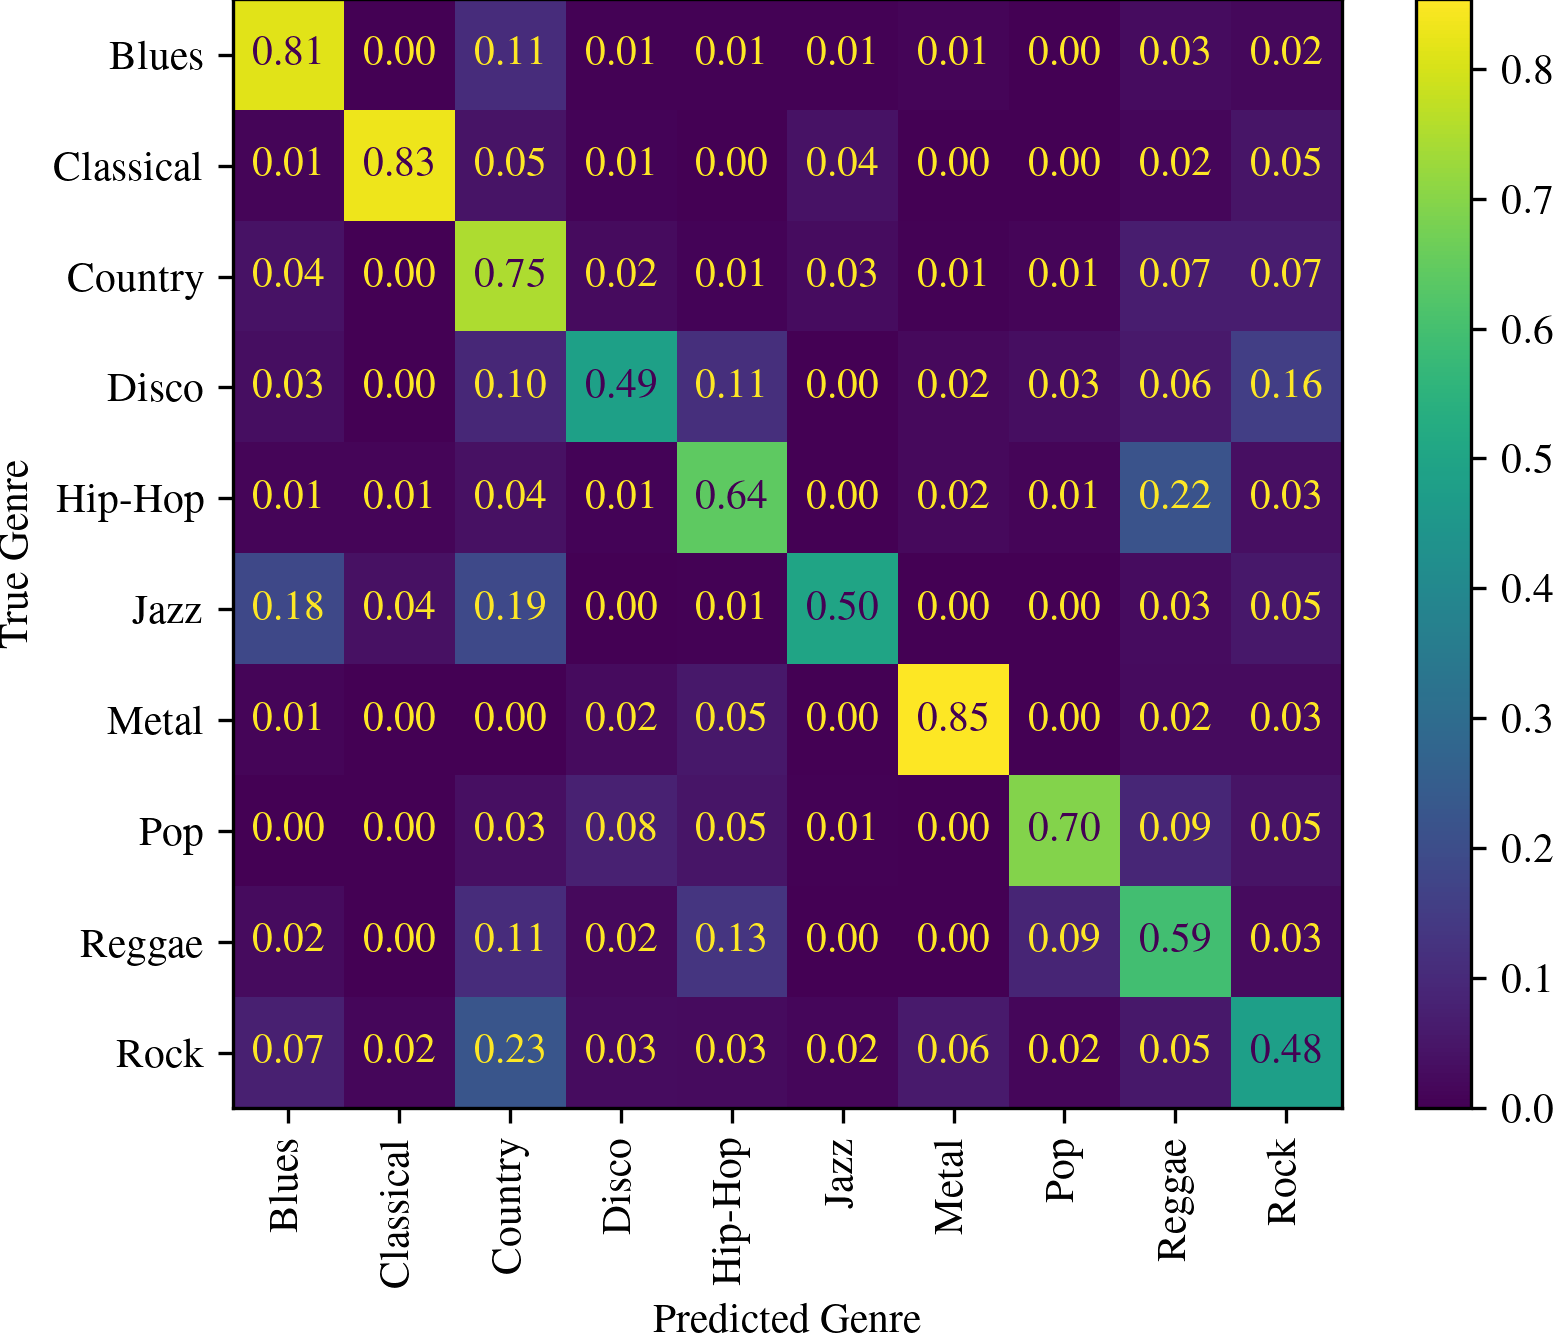
\includegraphics[width=\columnwidth]{cm.png}}
    \caption{
        Confusion matrix displaying the performance of my network on the test set after 200 epochs for a single training run.    
        The value in a given cell represents the proportion of samples from the true genre categorised as the predicted genre.
    }
    \label{confusion_matrix}
\end{figure}

\section{Training Curves}

Overfitting occurs when a network learns the random noise in the data as if it represents the structure of the underlying model.
To detect overfitting, I monitored the loss and accuracy of the network on both the training and test sets throughout the training process.
Figure \ref{accuracy_curves} and Figure \ref{loss_curves} display the accuracy and loss curves for the network, respectively.

\begin{figure}[htbp]
    \centerline{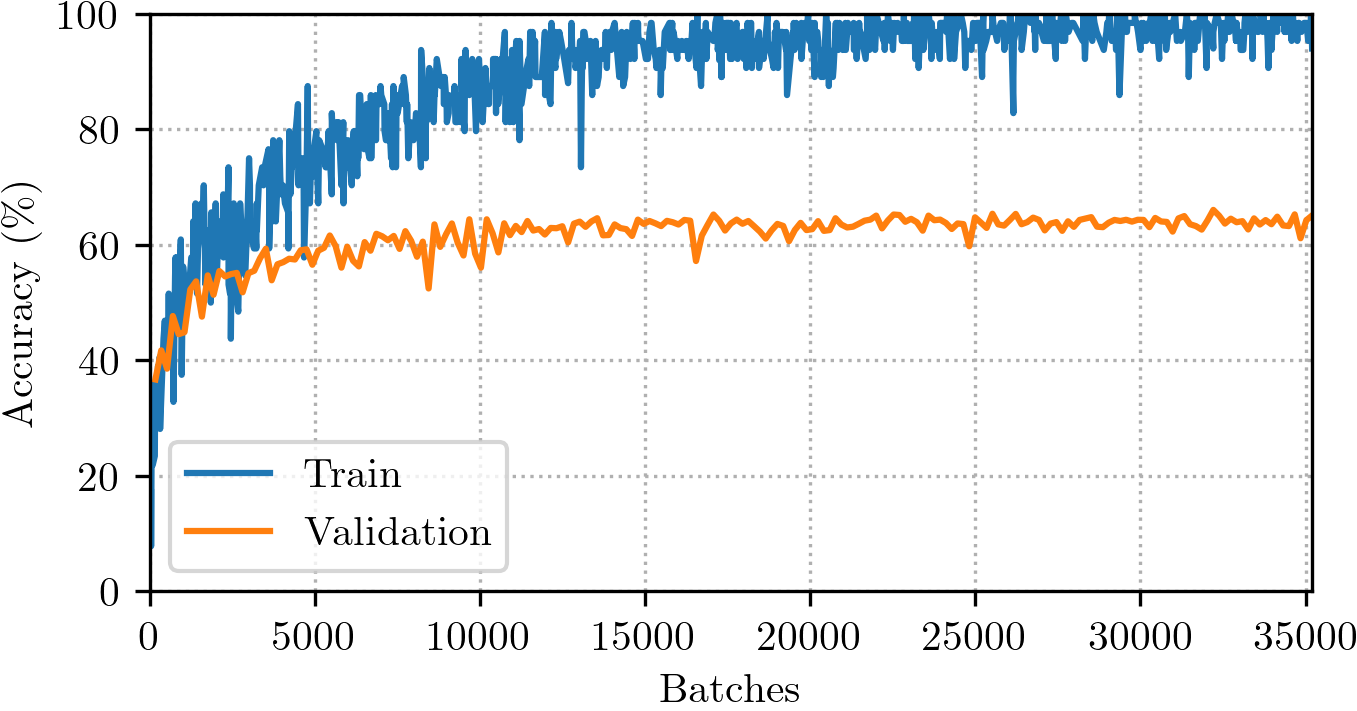
\includegraphics[width=\columnwidth]{accuracy.png}}
    \caption{
        Plot of accuracy data from the same training run as Figure \ref{confusion_matrix}.
        The line labelled `training' is the accuracy achieved on the training set, calculated every 100 batches; the line labelled `test' is the accuracy achieved on the test set, calculated every epoch.}
    \label{accuracy_curves}
\end{figure}

After 200 epochs, there was a significant difference of approximately 35\% in the model's accuracy on the training and test sets---this strongly indicates that the shallow CNN architecture had overfit the training data.
Even though I used L1 regularisation and dropout to mitigate overfitting, the model still memorised almost every sample in the training set and thus struggled to generalise to unseen data.

\begin{figure}[htbp]
    \centerline{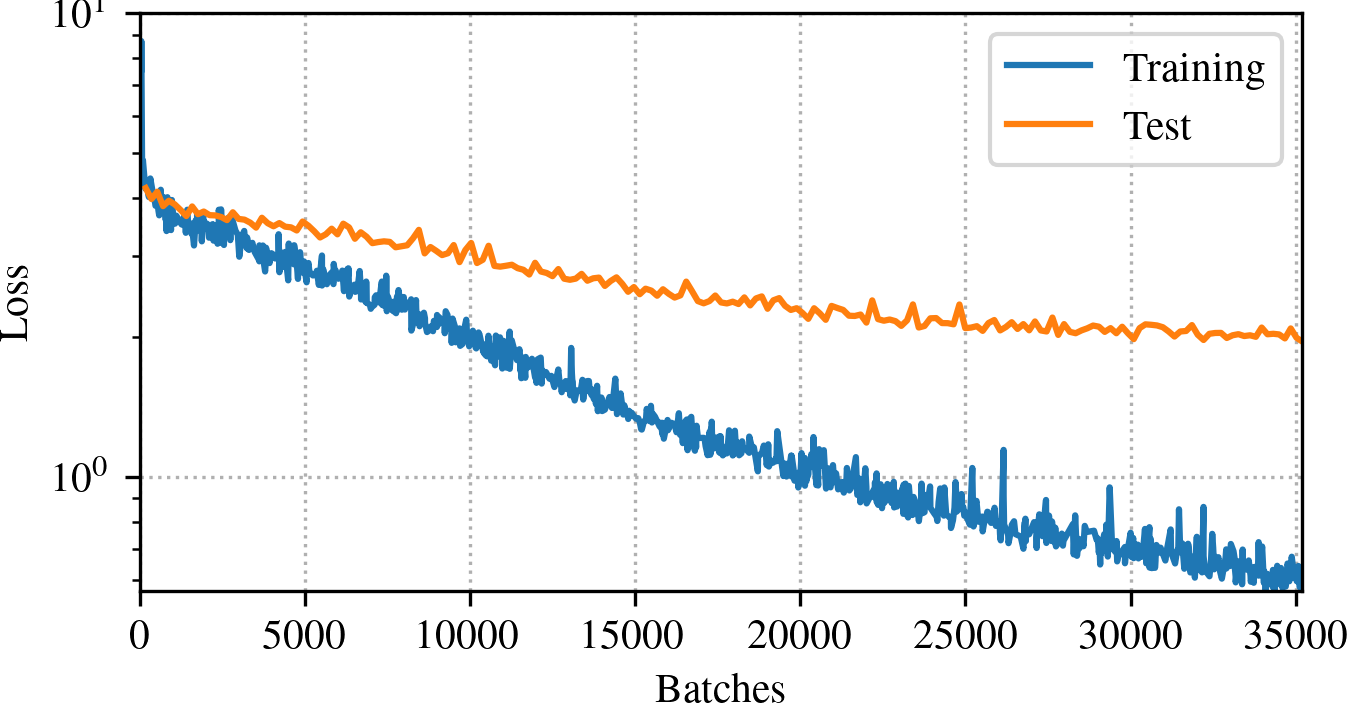
\includegraphics[width=\columnwidth]{loss.png}}
    \caption{
        Plot of loss data from the same training run as Figure \ref{confusion_matrix}.
        The line labelled `training' is the loss achieved on the training set, calculated every 100 batches; the line labelled `test' is the loss achieved on the test set, calculated every epoch.
    }
    \label{loss_curves}
\end{figure}

\section{Qualitative Results}

Deep neural networks are frequently described as black-box models because it can be challenging to reason about the features they extract to produce their outputs.
To provide a more comprehensive understanding of the network's performance, Figure \ref{spectrograms} presents three log-mel spectrograms produced from samples in the GTZAN dataset to illustrate where the network performed well and struggled.
By examining these spectrograms and listening to the corresponding audio files, I have gained an insight into the reasons for the discrepancies in per-class accuracy that the network achieved.

\begin{figure}[htbp]
    \centering
    \begin{subfigure}[b]{0.32\columnwidth}
        \centerline{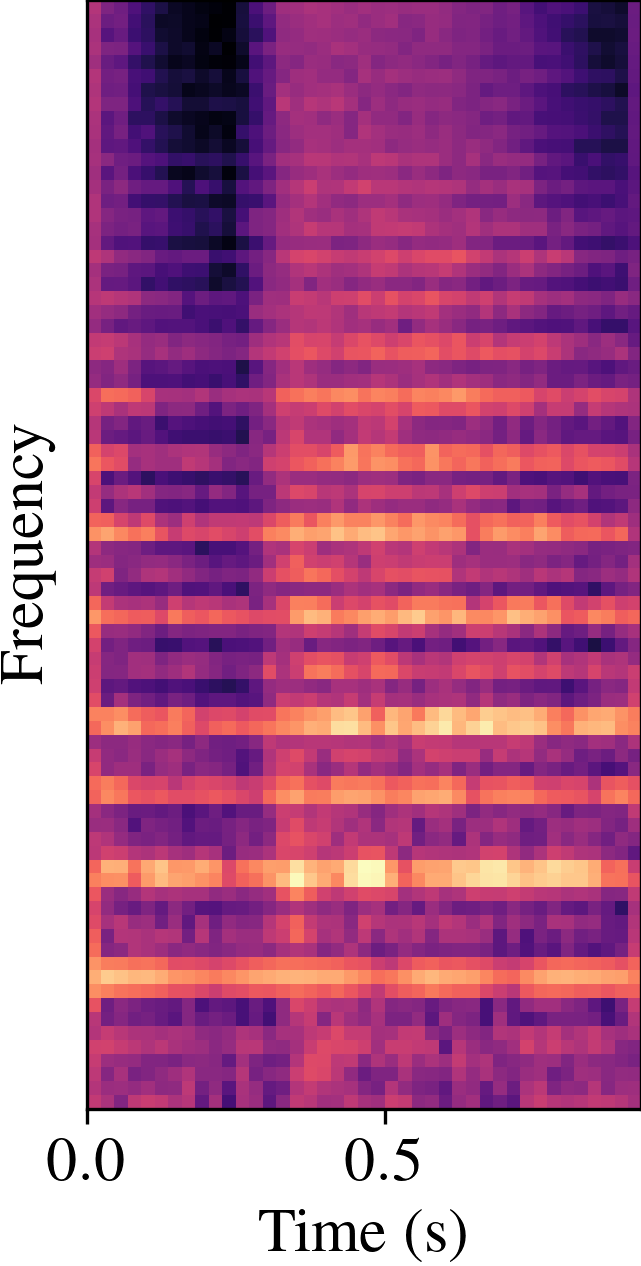
\includegraphics[width=\columnwidth]{spec_correct.png}}
        \caption{classical.00070.wav\\Ground truth: Classical\\Prediction: Classical}
        \label{spec_correct}
    \end{subfigure}
    \hfill
    \begin{subfigure}[b]{0.32\columnwidth}
        \centerline{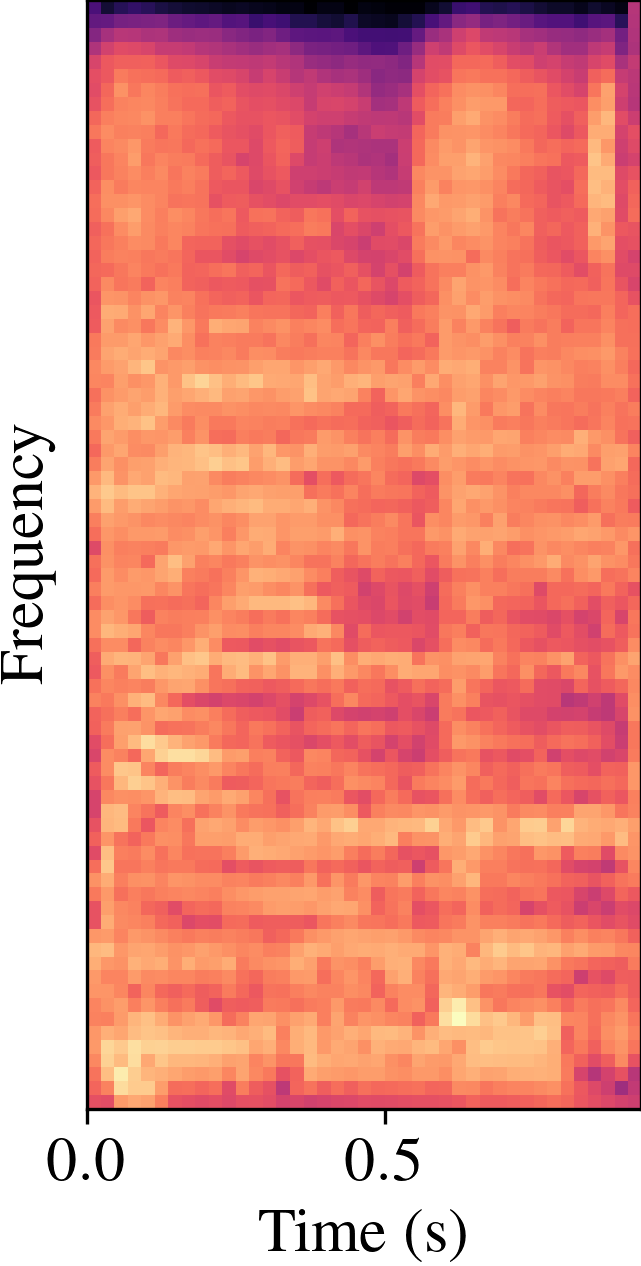
\includegraphics[width=\columnwidth]{spec_incorrect_1.png}}
        \caption{jazz.00003.wav\\Ground truth: Jazz\\Prediction: Classical}
        \label{spec_incorrect_1}
    \end{subfigure}
    \hfill
    \begin{subfigure}[b]{0.32\columnwidth}
        \centerline{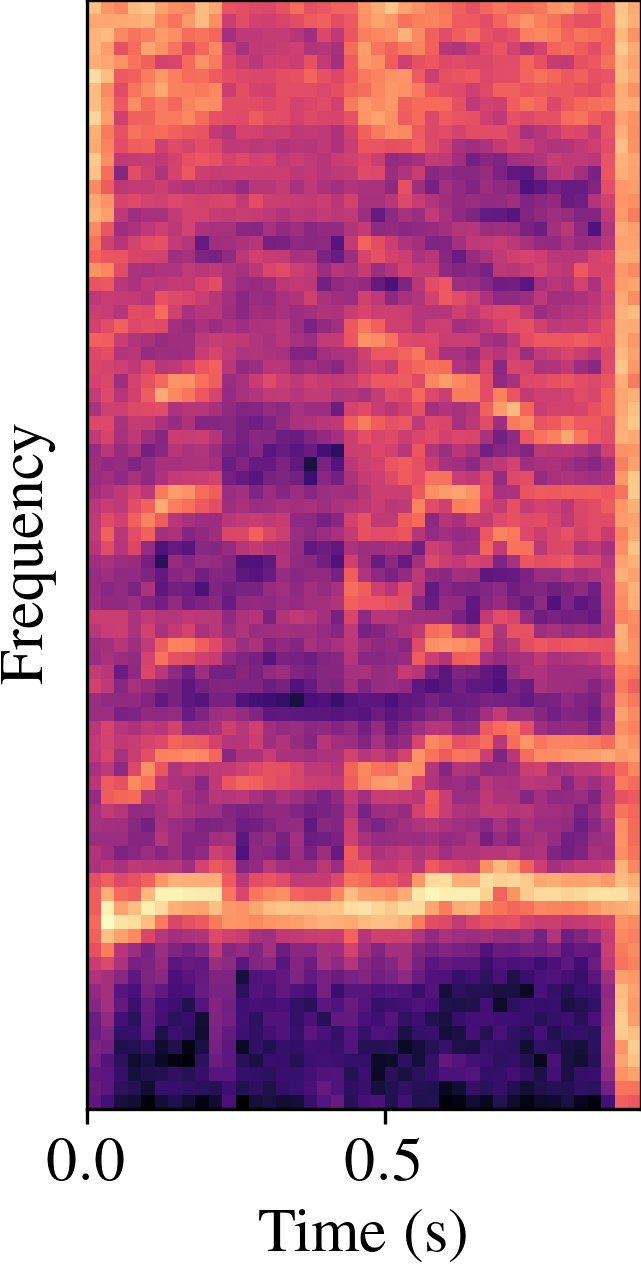
\includegraphics[width=\columnwidth]{spec_incorrect_2.png}}
        \caption{pop.00064.wav\\Ground truth: Pop\\Prediction: Disco}
        \label{spec_incorrect_2}
    \end{subfigure}
    \caption{
        Log-mel spectrograms produced from three audio files in the test dataset.
        Under each spectrogram is the name of the audio file the spectrogram is from, the ground-truth genre, and the predicted genre.
    }
    \label{spectrograms}
\end{figure}

Figure \ref{spec_correct} displays a correctly classified spectrogram from the classical genre.
The network correctly classified all 15 spectrograms produced from the same audio file.
The network's high performance on this file is unsurprising, as the music from the file is very typical of classical music, with the string section of an orchestra playing the piece.
The harmonics these string instruments produce are clearly visible in the spectrogram as extended parallel lines.

In contrast, Figure \ref{spec_incorrect_1} displays a spectrogram from a piece of jazz music that the network misclassified as classical.
It made the same error with 9 of the 15 spectrograms derived from the same piece of music.
Although it is impossible to determine the exact reason for these errors, the music itself appeared to borrow elements from both the classical and jazz genres.
While the piece uses a jazz chord progression, there is no syncopated beat, and it appears to contain a classical drum.
Therefore, if a spectrogram was produced from a short sample that included a classical drum, for example, it is not surprising that the network misclassified it.
The misclassification suggests that the short duration used to produce each log-mel spectrogram likely degrades the overall accuracy of the network.
It highlights a potential problem with the overall method, in that 0.93-second samples are often insufficient to accurately represent a piece of music.

Figure \ref{spec_incorrect_2} shows a spectrogram produced from pop music that the network misclassified as disco.
However, the song the spectrogram was produced from has a disco beat, and the first set of vocals is typical of disco music.
This blending of genres is not uncommon---disco music has influenced many modern pop songs, and pop artists often incorporate disco elements into their music.
Arguably, this highlights a potentially fundamental issue with classifying using genre in the first place.
The concept of genre is somewhat subjective and can vary depending on the individual and their taste.
Many pieces of music fit into multiple genres, and this piece likely fits into that category.

\section{Improvements}

\subsection{Maximum Probability and Majority Voting}

As previously mentioned, each audio file in the GTZAN \cite{TzanetakisCook} dataset was preprocessed to produce 15 log-mel spectrograms.
In order to improve the accuracy of the network, I implemented two additional classification methods that take these file dependencies into account: maximum probability classification and majority vote classification.
\begin{itemize}
    \item Maximum probability: the probabilities output by the final softmax layer for each spectrogram are first summed. The largest value amongst the summed probabilities then determines the predicted class.
    \item Majority vote: a class is determined for each spectrogram by the largest value output by the final layer. A majority vote is then conducted over the predicted classes for each segment.
\end{itemize}

Table \ref{improved_results} displays the mean accuracy of the raw, maximum probability and majority vote approaches on the test set over five runs.
The relative improvement in accuracy provided by the two new approaches is consistent with the findings of Schindler et al. in \cite{SchindlerLidyRauber}.
Moreover, including all three accuracy metrics makes the findings more comparable with the broader literature, which frequently employs these three approaches.

\begin{table}[htbp]
    \caption{Improved accuracy achieved on the test set}
    \begin{center}
    \begin{tabular}{l c c c c}
    \toprule
    &&\multicolumn{3}{c}{\textbf{Accuracy}}\\
    \cmidrule(lr){3-5}
    \textbf{Model}&\textbf{Epoch}&\textbf{Raw}&\textbf{Max}&\textbf{Maj}\\
    \midrule
    \multirow{ 2}{*}{My CNN} & 100 & 63.28 & 77.44 & 75.84 \\
    & 200 & 64.22 & 77.20 & 76.16 \\
    \midrule
    \multirow{ 2}{*}{My CNN + Batch Norm} & 100 & 66.57 & 78.88 & 76.24 \\
    & 200 & \textbf{66.78} & \textbf{79.60} & \textbf{77.68} \\
    \bottomrule
    \end{tabular}
    \label{improved_results}
    \end{center}
\end{table}

These methods allow the network to consider the collective evidence from all the spectrograms for each audio file to make a more informed and accurate prediction about the genre.
The increase in accuracy is due to there being some amount of independence in the predictions of samples from a given file.
This independence can be attributed to the 0.93-second samples often being too short to be representative and the model overfitting the training data.
The majority vote and maximum probability classification methods effectively eliminate many individual errors to produce more accurate and informed predictions for entire files.

\subsection{Batch Normalisation}

Batch normalisation \cite{IoffeSzegedy} is frequently employed to increase the speed and stability of the training process.
It consists of a normalisation step that fixes the means and variances of each layer's input.

I implemented a two-dimensional batch normalisation layer following the network's two convolutional layers.
Table \ref{improved_results} displays the mean accuracy of the network on the test set over five runs with the inclusion of the batch normalisation layers; it shows that batch normalisation provided approximately a 2\% increase in accuracy across all three classification methods.
There is disagreement in the broader literature on deep learning regarding the precise mechanisms for batch normalisation's empirically substantial benefits.
Santukar et al. \cite{SanturkarEtAl} identified that the batch normalisation layers significantly smooth the optimisation landscape, thus inducing a more predictive and stable behaviour of the gradients, which facilitates faster training and enables the model to converge to a better solution.

Batch normalisation also has a regularising effect that helps mitigate overfitting, as seen in Figure \ref{accuracy_curves_improved}.
Unlike with the network trained without batch normalisation, the network did not consistently hit 100\% accuracy on the test set, and the discrepency in accuracy between the training and test set was lower at each stage.
The regularising effect can be attributed to each mini-batch having a slightly different mean and standard deviation, thus causing the batch normalisation layers to normalise each slightly differently.
As such, there is an element of randomness, which encourages the network to be less sensitive to the random noise in its input.
This overall mitigates the degree to which the network overfits.

\begin{figure}[htbp]
    \centerline{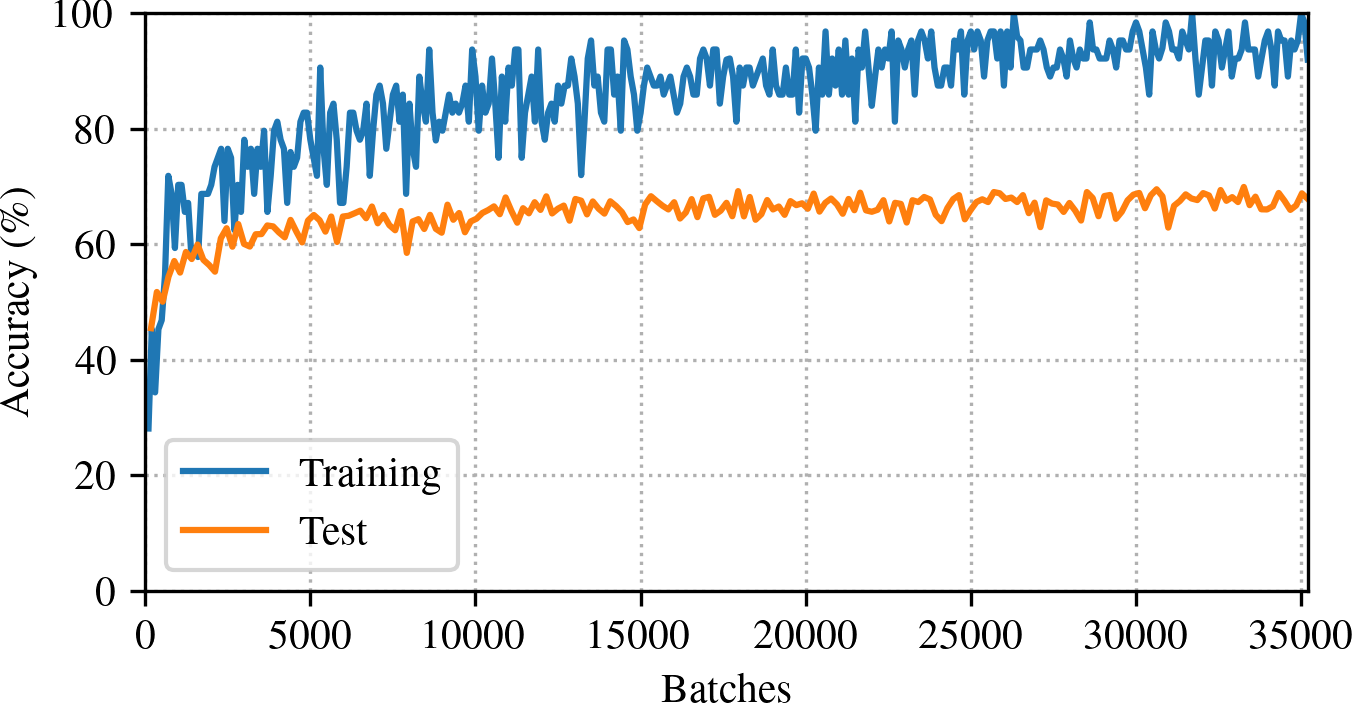
\includegraphics[width=\columnwidth]{accuracy_improved.png}}
    \caption{
        Plot of accuracy data for the improved network from a single training run.
        Format is the same as for Figure \ref{accuracy_curves}.
    }
    \label{accuracy_curves_improved}
\end{figure}

Figure \ref{confusion_matrix_improved} displays a confusion matrix displaying the improved performance of the network following the implementation of batch normalisation.
The network classified samples on a per-file basis using the maximum probability method.
There is an evident improvement in per-class accuracy across the genres.
Notably, the network accurately classified 100\% of audio files from the classical genre.
However, while the improved performance has eliminated many of the smaller (e.g. $\approx 1\%$) misclassifications for specific genres, there are still some significant errors.
For example, the network still misclassified approximately 20\% of reggae songs as hip-hop

\begin{figure}[htbp]
    \centerline{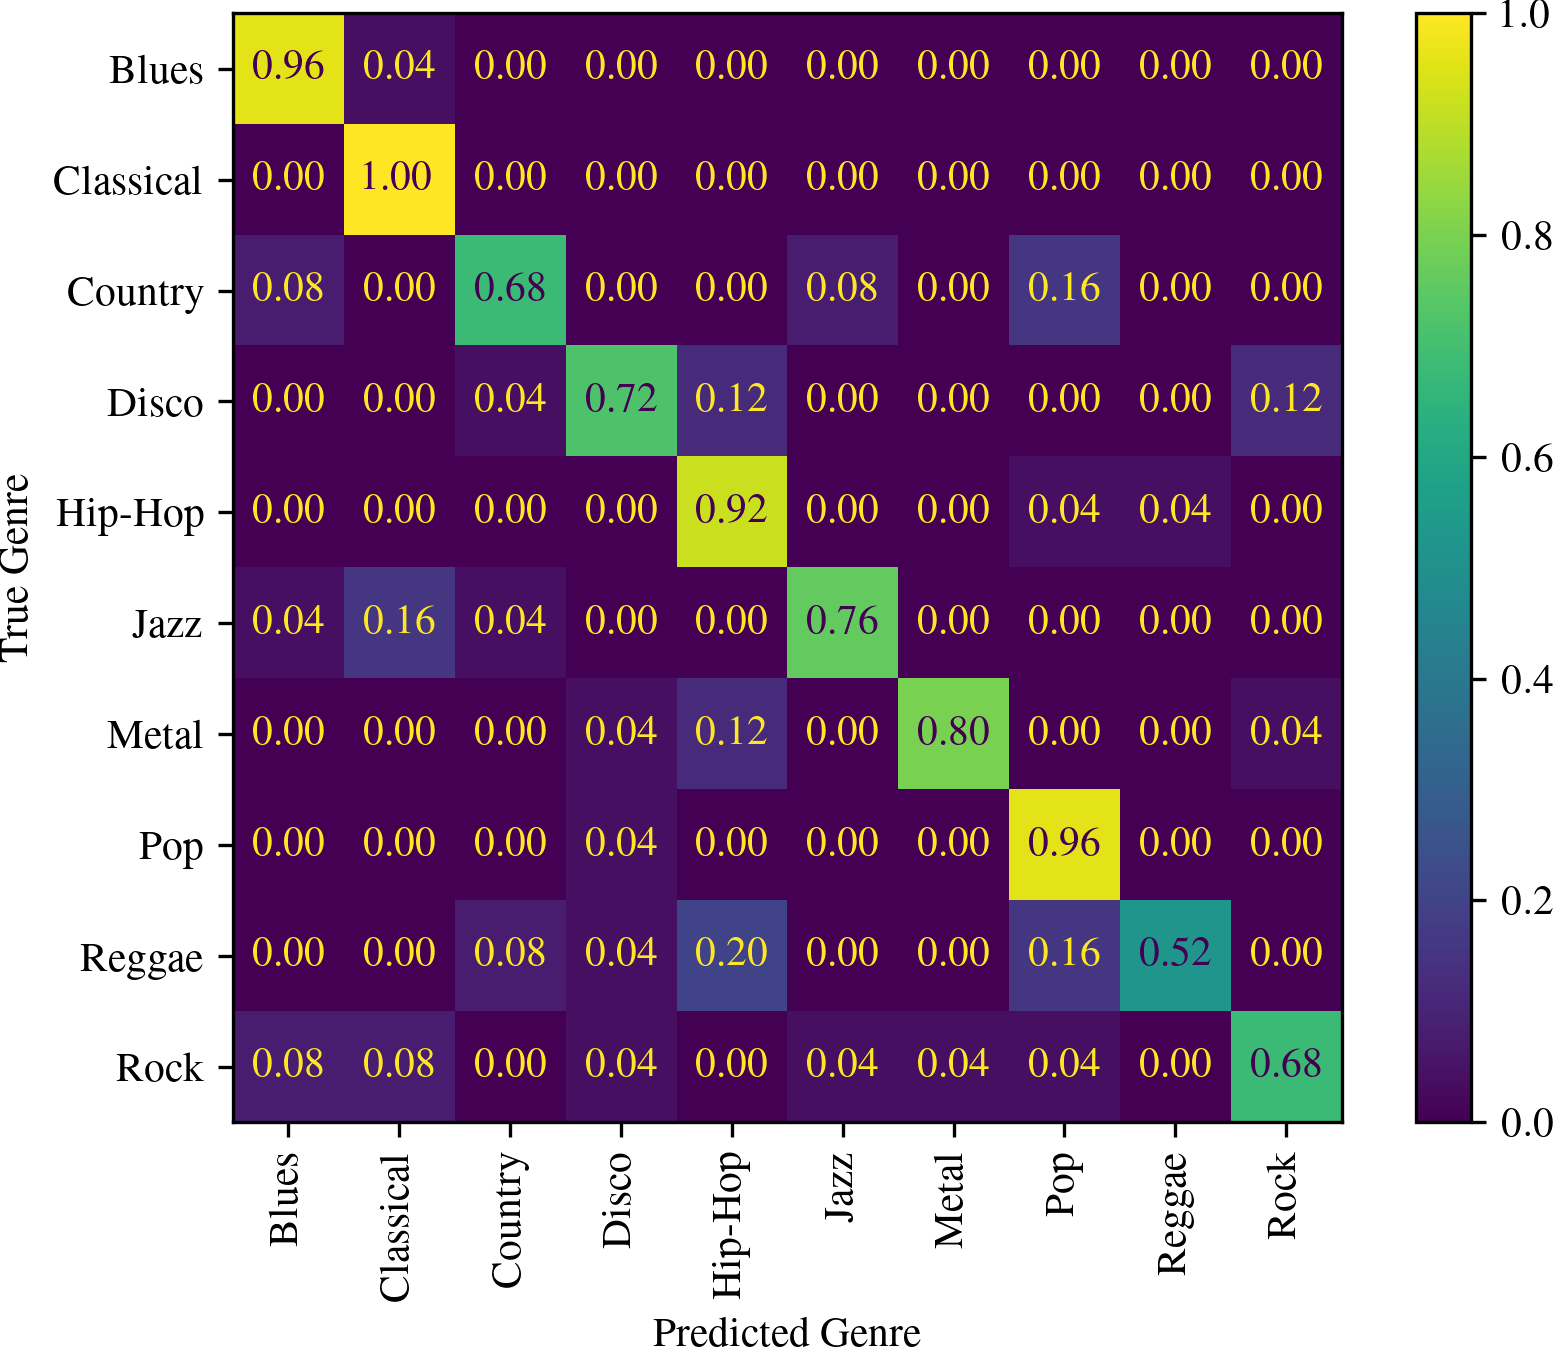
\includegraphics[width=\columnwidth]{cm_improved.png}}
    \caption{
        Confusion matrix displaying the performance of the improved network with batch normalisation on the test set after 200 epochs for a single training run.
        Classification was performed using the maximum probability method.
        Format is the same as for Figure \ref{confusion_matrix}.
    }
    \label{confusion_matrix_improved}
\end{figure}

\section{Conclusion and Future Work}

This paper has described a reimplementation of the shallow CNN architecture as published originally by Schindler et al. in \cite{SchindlerLidyRauber} for genre classification.
The network has been trained and evaluated on the GTZAN \cite{TzanetakisCook} dataset, a much-used dataset in the broader literature.
I have built on the analysis conducted by Schindler et al., describing a significant discrepancy in the per-class accuracy achieved by the model that was not reported in the original work.
I have also conducted an extensive qualitative analysis to understand where the network performs well and fails.
Notably, I identified several failure cases that suggest potential issues with the method, in that 0.93-second samples are often too short to be representative, as well as the use of genre to classify owing to its partially subjective nature.

In the latter part of this paper, I have also proposed an extension to the architecture with the inclusion of two batch normalisation layers.
Including two batch normalisation layers enabled the network to be trained significantly faster and converge to a better solution.

The improvements achieved via the inclusion of the batch normalisation layers naturally invite several avenues to explore in future work.
For example, further studies could investigate the inclusion of group normalisation \cite{WuKaiming} layers, which several studies have shown to offer an advantage over batch normalisation in several computer vision networks.

\bibliographystyle{IEEEtran}
\bibliography{refs}

\end{document}
